\subsection{Inseparable points}
\label{sec: knnInSep}

\begin{figure}
\hfill
\subfigure[Default]{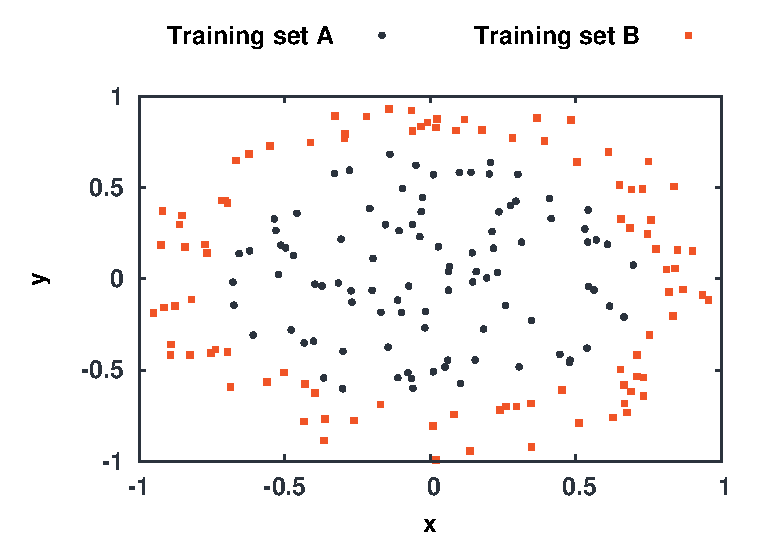
\includegraphics[width=0.48\textwidth]{figures/knn_95_55_inseparable_default_weighted_samples.eps} \label{fig: knnInSepTrainSetDef}}
\hfill
\subfigure[Distant]{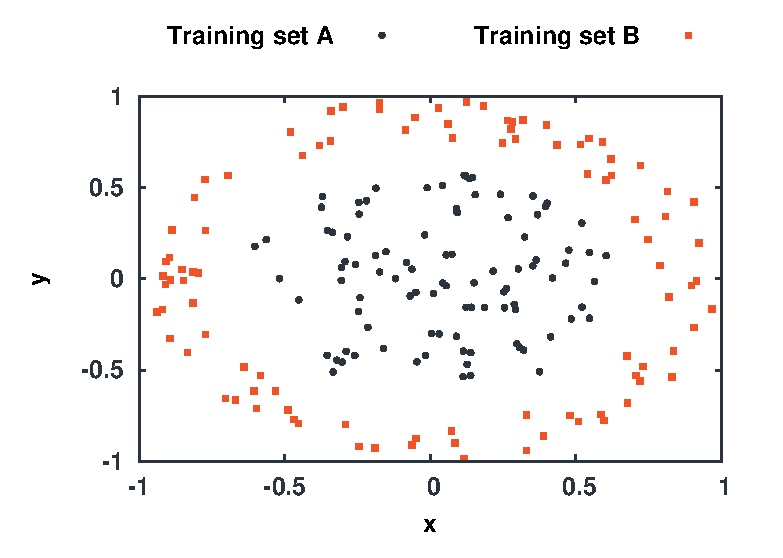
\includegraphics[width=0.48\textwidth]{figures/knn_95_55_inseparable_distant_weighted_samples.eps} \label{fig: knnInSepTrainSetDis}}
\hfill
\centering\subfigure[Overlapped]{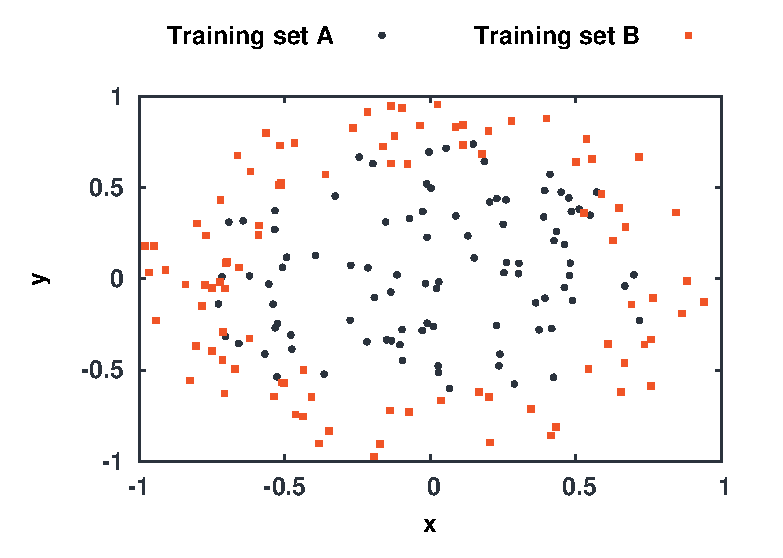
\includegraphics[width=0.48\textwidth]{figures/knn_95_55_inseparable_overlapped_weighted_samples.eps} \label{fig: knnInSepTrainSetOvr}}
\hfill
\caption{Training sets for inseparable points (inside / outside a circle).}
\label{fig: knnInSepTrainSet}
\end{figure}

Lets now consider points which are not linearly separable, i.e. points inside and outside a circle, as presented on Fig. \ref{fig: knnInSepTrainSet}. Once again, three cases are investigated: default (points exactly separated by a circle, Fig. \ref{fig: knnInSepTrainSetDef}), distant (with extra gap between training sets, Fig. \ref{fig: knnInSepTrainSetDis}), and overlapped (training sets are allowed to overlap a little, Fig. \ref{fig: knnInSepTrainSetOvr}).

\begin{figure}
\hfill
\subfigure[Default, unweighted]{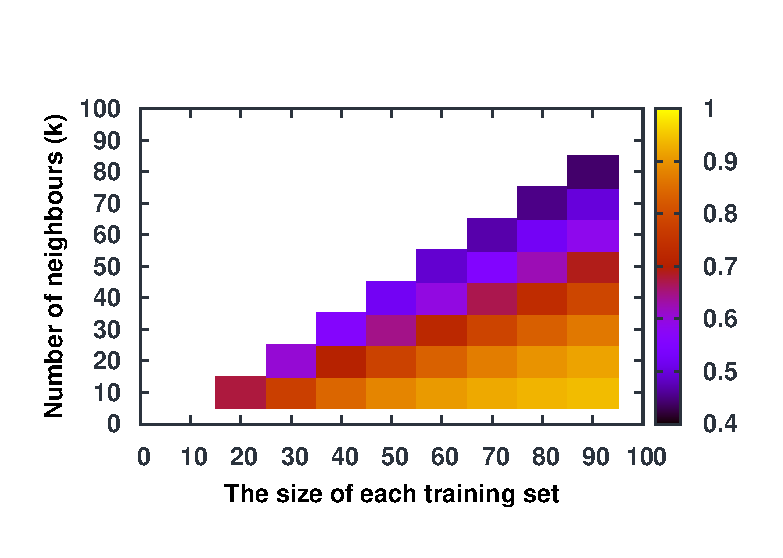
\includegraphics[width=0.48\textwidth]{figures/knn_inseparable_default_unweighted.eps} \label{fig: knnInSepResDefU}}
\hfill
\subfigure[Default, weighted]{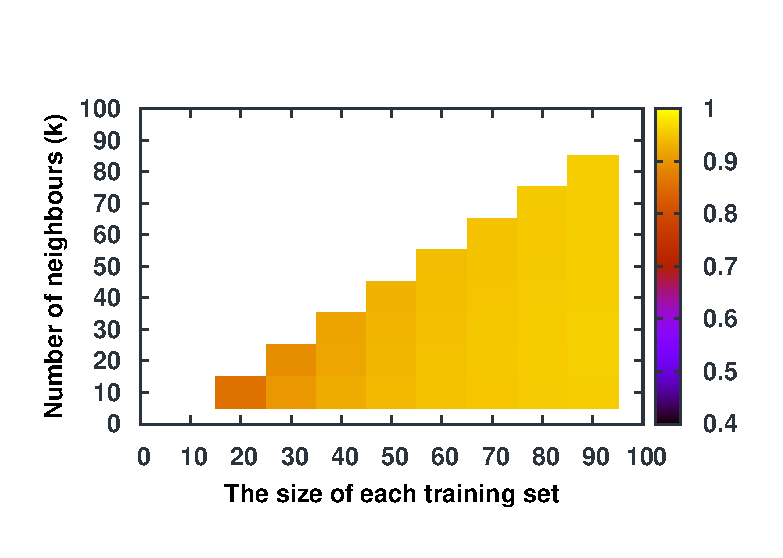
\includegraphics[width=0.48\textwidth]{figures/knn_inseparable_default_weighted.eps} \label{fig: knnInSepResDefW}}
\hfill
\subfigure[Distant, unweighted]{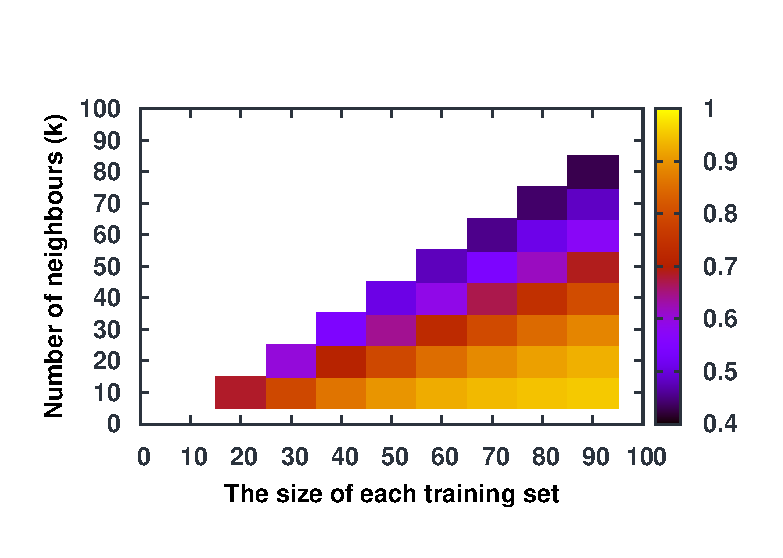
\includegraphics[width=0.48\textwidth]{figures/knn_inseparable_distant_unweighted.eps} \label{fig: knnInSepResDisU}}
\hfill
\subfigure[Distant, weighted]{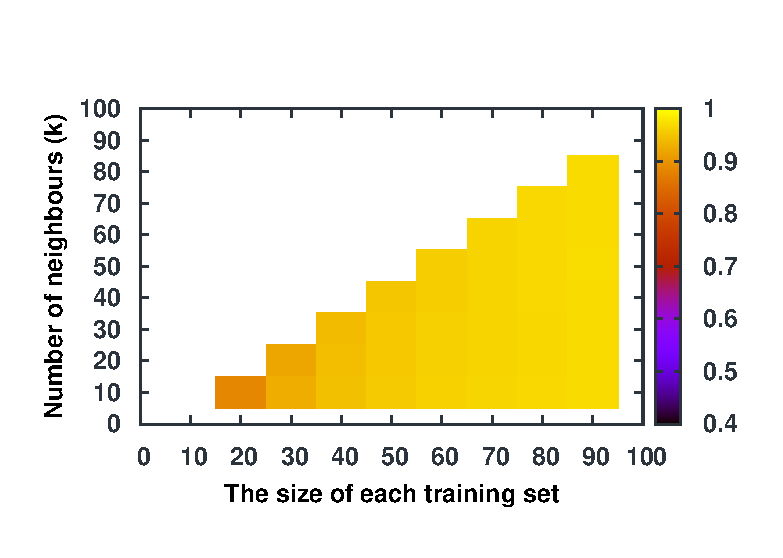
\includegraphics[width=0.48\textwidth]{figures/knn_inseparable_distant_weighted.eps} \label{fig: knnInSepResDisW}}
\hfill
\subfigure[Overlapped, unweighted]{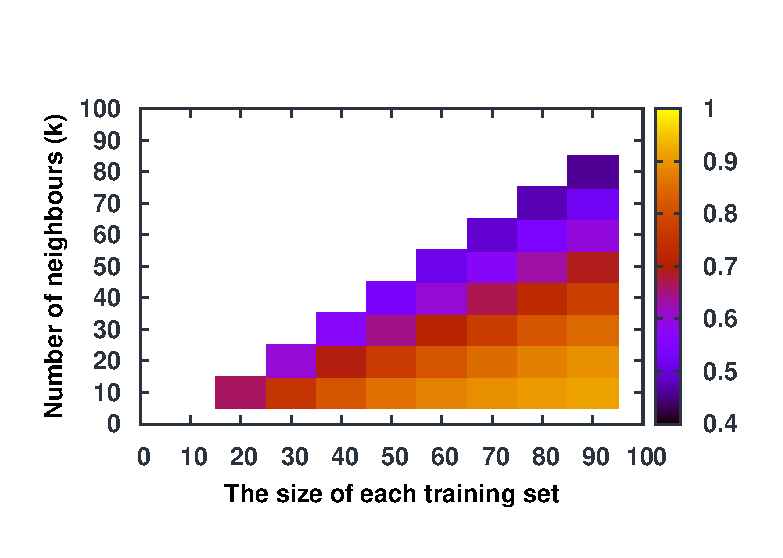
\includegraphics[width=0.48\textwidth]{figures/knn_inseparable_overlapped_unweighted.eps} \label{fig: knnInSepResOvrU}}
\hfill
\subfigure[Overlapped, weighted]{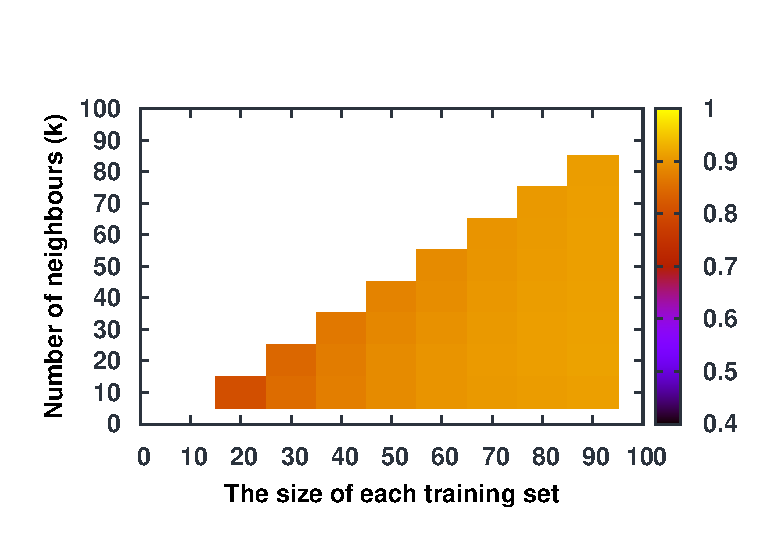
\includegraphics[width=0.48\textwidth]{figures/knn_inseparable_overlapped_weighted.eps} \label{fig: knnInSepResOvrW}}
\hfill
\caption{kNN efficiency for inseparable points.}
\label{fig: knnInSepRes}
\end{figure}

The efficiency, presented on Fig. \ref{fig: knnInSepRes}, is calculated exactly the same way as in Sec. \ref{sec: knnSep}. Please note the different scale which now starts at $0.4$. Clearly, unweighted kNN requires now larger training sets to get an efficiency $\geq 90\%$. It is expected, though. The more complex problem the larger training set is necessary. Weighted kNN still works (surprisingly?) pretty well even for small training sets.